\section{Results}\label{sec:results}

To get a finer intuition about the results, we show  some visual examples, separated in two groups of Figures. The first group, shows the mean value achieved by the GA given a function. The second one, shows the convergence plot with the mean of the values found at each generation, the function target value with a given tournament size.

All Figures represent the mean of 40 repetitions given a certain dimension.

To better understand the results, we performed the Friedman Test analysis over all optimum values achieved from the GA.% These optimum values represent the values obtained from the 1728 different combinations paired by the 24 functions, the 3 dimensions and the 24 tournament sizes.




\subsection{First Group}
The Figures~\ref{5dim_10},~\ref{5dim_20},~\ref{5dim_40},~\ref{12dim_10},~\ref{12dim_20},~\ref{12dim_40},~\ref{21dim_10},~\ref{21dim_20} and~\ref{21dim_40} exemplify that for the F5, F12, and F21 function (with 10, 20 and 40 dimensions) that changing the tournament size, does not lead to significant better final values found by the GA. The gray shaded area represents the 95\% confidence level interval for predictions from a linear model for each scenario showed. For all Figures, the mean of 40 repetitions is shown as bullets and the bars represent the standard deviation, with 40 dimensions.


\begin{figure}[H]
	\includegraphics[width=0.5\textwidth]{img/5dim_10.ps}
	\caption{Optimum values for the F5 function by the GA.}
	\label{5dim_10}
\end{figure}

\begin{figure}[H]
	\includegraphics[width=0.5\textwidth]{img/5dim_20.ps}
	\caption{Optimum values for the F5 function by the GA.}
	\label{5dim_20}
\end{figure}

\begin{figure}[H]
	\includegraphics[width=0.5\textwidth]{img/5dim_40.ps}
	\caption{Optimum values for the F5 function by the GA.}
	\label{5dim_40}
\end{figure}

\begin{figure}[H]
	\includegraphics[width=0.5\textwidth]{img/12dim_10.ps}
	\caption{Optimum values for the F12 function by the GA.}
	\label{12dim_10}
\end{figure}

\begin{figure}[H]
	\includegraphics[width=0.5\textwidth]{img/12dim_20.ps}
	\caption{Optimum values for the F12 function by the GA.}
	\label{12dim_20}
\end{figure}

\begin{figure}[H]
	\includegraphics[width=0.5\textwidth]{img/12dim_40.ps}
	\caption{Optimum values for the F12 function by the GA.}
	\label{12dim_40}
\end{figure}



\begin{figure}[H]
	\includegraphics[width=0.5\textwidth]{img/21dim_10.ps}
	\caption{Optimum values for the F21 function by the GA.}
	\label{21dim_10}
\end{figure}

\begin{figure}[H]
	\includegraphics[width=0.5\textwidth]{img/21dim_20.ps}
	\caption{Optimum values for the F21 function by the GA.}
	\label{21dim_20}
\end{figure}

\begin{figure}[H]
	\includegraphics[width=0.5\textwidth]{img/21dim_40.ps}
	\caption{Optimum values for the F21 function by the GA.}
	\label{21dim_40}
\end{figure}

\subsection{Second Group}
The Figure~\ref{convegenceF1} exemplifies that for the F1 function (with 10 dimensions), the GA is converging towards the optimum target value, represented by the red, vertical line. 

\begin{figure}[!ht]
	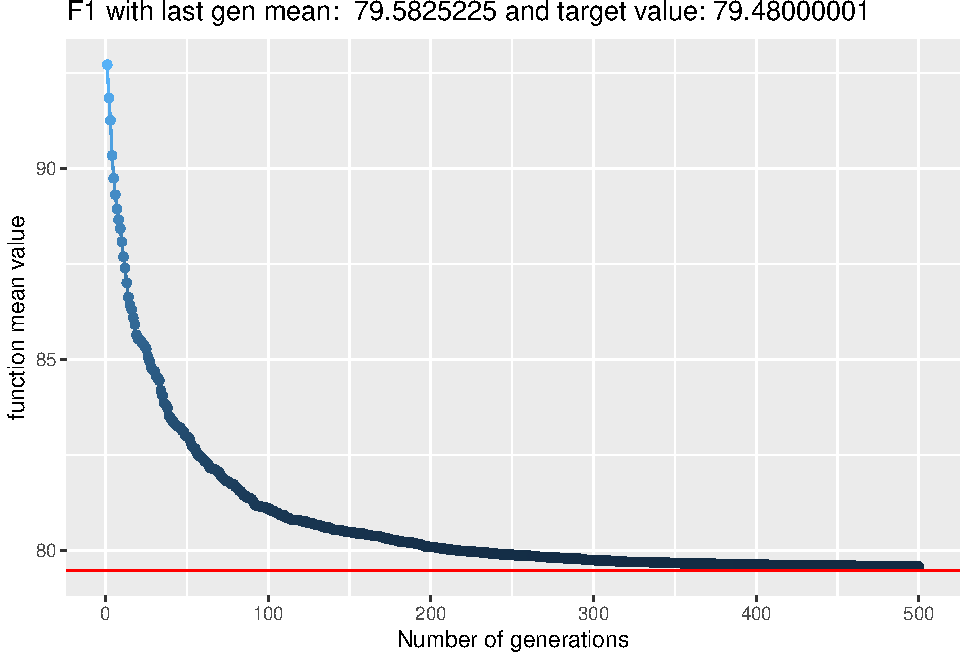
\includegraphics[width=0.5\textwidth]{img/unnamed-chunk-1-1}
	\caption{Population convergence for function F1. The mean of 40 repetitions is shown, with 40 dimensions.}
	\label{convegenceF1}
\end{figure}


\subsection{Friedman Test Analysis}
The Friedman Test analysis showed that, as expected, there was no significant difference in values among tournament size values. The test was performed with the results obtained with 10, 20 and 40 dimensions, given the 24 BBOB benchmark functions. Detailed data can be visualized on the following Table~\ref{Friedman_test}. 

\vspace{3mm}
\begin{table}[!ht]
	\centering
	\label{Friedman_test}
	\begin{tabular}{|l|l|l|}
		\hline
		Dimension size      & Chi-squared        & P-value                     \\ \hline
		\multicolumn{1}{|l|}{10} & \multicolumn{1}{l|}{31.497} & \multicolumn{1}{l|}{0.1111} \\ \hline
		\multicolumn{1}{|l|}{20} & \multicolumn{1}{l|}{27.903} & \multicolumn{1}{l|}{0.2195} \\ \hline
		\multicolumn{1}{|l|}{40} & \multicolumn{1}{l|}{23.288} & \multicolumn{1}{l|}{0.444}  \\ \hline
	\end{tabular}
	\caption{Friedman Test results, with the dependent variable being the value obtained, the blocking variables are the functions and the treatment variable is the tournament size value.}

\end{table}